\documentclass[dvipdfmx,12pt]{beamer}
%\documentclass[dvipdfmx,12pt,handout]{beamer}
\usepackage{pxjahyper}
\usepackage{minijs}
\usepackage{otf}
\renewcommand{\kanjifamilydefault}{\gtdefault}
\useoutertheme{infolines}
\usecolortheme[RGB={0,128,0}]{structure}
\usecolortheme{dolphin}
\setbeamertemplate{navigation symbols}{}
\setbeamercolor{frametitle}{fg=white, bg=gray}

\title{Auction For Complements}
\author{小川慶将}
\date{\today}

\begin{document}
\begin{frame}\frametitle{}
 \titlepage
\end{frame}

\begin{frame}\frametitle{発表の流れ}
 \tableofcontents
\end{frame}

\section{前回の復習}
\subsection{シングルオークション}
\begin{frame}
\frametitle{シングルオークションとは}
\begin{itemize}\setlength{\parskip}{0.5em}
\item
主に4種に分類される。
\begin{itemize}\setlength{\parskip}{0.5em}
\item
イングリッシュ・オークション(価格上昇オークション)
\item
ダッチ・オークション(価格下落オークション)
\item
ファーストプライス封印オークション
\item
セカンドプライス封印オークション
\end{itemize}
\end{itemize}
\end{frame}


\subsection{ダブルオークション}
\begin{frame}
\frametitle{ダブルオークションとは}
\begin{itemize}\setlength{\parskip}{0.5em}
\item
売り手も買い手も複数人存在する市場。\\
株取引などで使われる。\pause
\item
前回未完成だったプログラムが完成しました。\\
けど日本語に不備あり。笑
\end{itemize}
\end{frame}

\section{複数財オークション}
\subsection{複数財オークションとは}
\begin{frame}
\frametitle{複数財オークションとは}
\begin{itemize}\setlength{\parskip}{0.5em}
\item
今までのオークションと違って異種複数財を扱うオークション。\\
財1と財2を一緒に買うことで相乗効果が生まれたりする。\pause
\item
遊戯王のエグゾディアとかそれなのか?笑
\end{itemize}
\begin{figure}
\centering
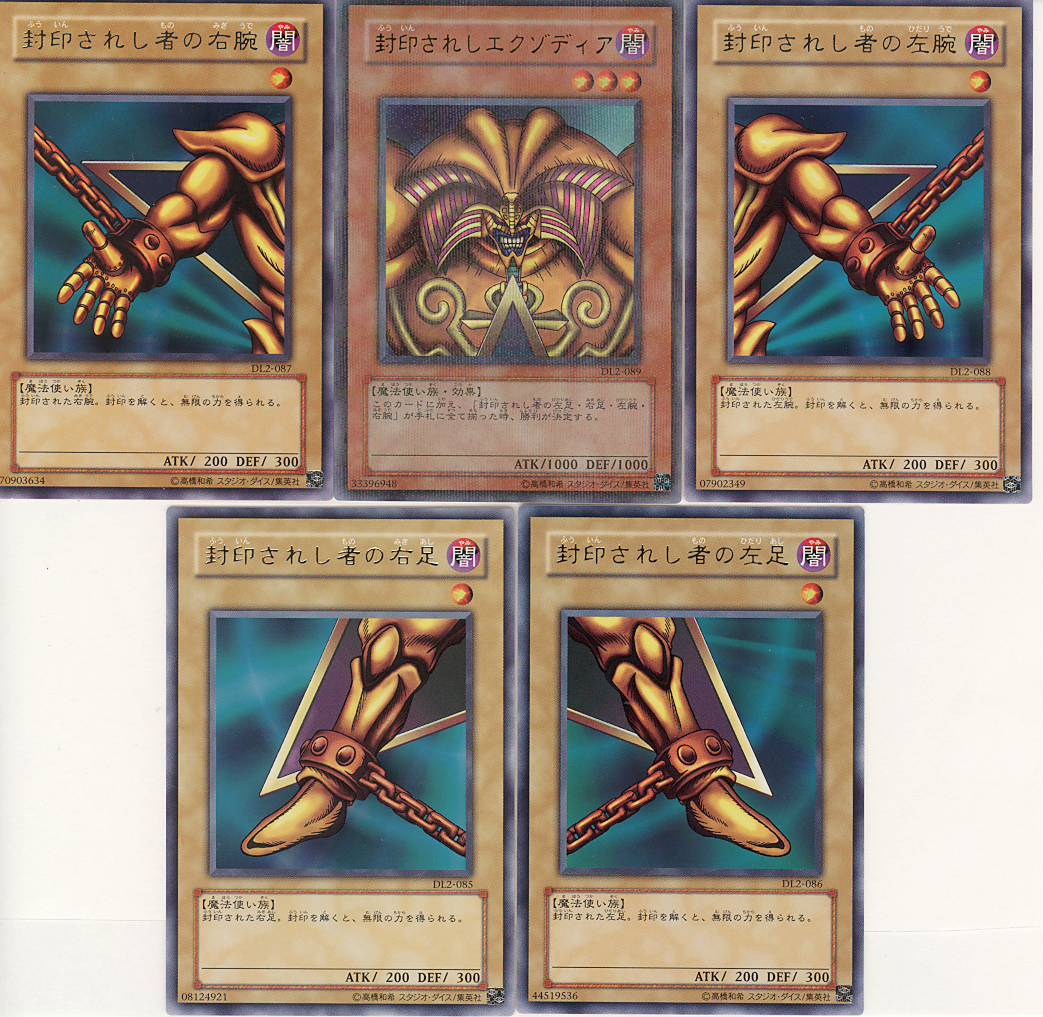
\includegraphics[width=50mm]{yuugi.jpg}
\label{fig:jukyuu}
\end{figure}
\end{frame}


\subsection{Let's 実験}
\begin{frame}
\frametitle{実験開始}
\begin{itemize}\setlength{\parskip}{0.5em}
\item
とりあえずまず実験してみよう。
\end{itemize}
\end{frame}

\subsection{}
\begin{frame}
\frametitle{実験デザインの種類}
\begin{itemize}\setlength{\parskip}{0.5em}
\item
複数財オークションにおいて主に4つの実験デザインがある。\pause
\begin{itemize}\setlength{\parskip}{0.5em}
\item
The First Price Auction\pause
\item
Vickrey Auction\pause
\item
The Vickrey Nearest Rule\pause
\item
The Reference Rule Auction\pause
\end{itemize}
\item
今回はFPとVAとRRで実験を行った。
\end{itemize}
\end{frame}

\begin{frame}
\frametitle{The First Price Auction}
\begin{itemize}\setlength{\parskip}{0.5em}
\item
自分が出したビッド額がそのまま自分が払う価格になる。\pause
\item
数式で表す以下の通り。
\begin{equation}
P^{FP}(b_{i1}, b_{i2}, b_{j}) = \begin{cases}
    (b_{i1}, b_{i2}, 0) & (b_{i1} + b_{i2} >= b_{j}) \\
    (0, 0, b_{j}) & (b_{i1} + b_{i2} < b_{j})
  \end{cases}
\end{equation}\pause
\item
例:(200, 300, 400)のときI1-typeが200円、I2-typeが300円で落札する。\pause
\item
最適反応は相手のビッド額のちょっと上をビッドすること。\pause
\item
真の評価額を引き出して売り手の収益を最大にするデザインが欲しい!
\end{itemize}
\end{frame}

\begin{frame}
\frametitle{Vickrey Auction}
\begin{itemize}\setlength{\parskip}{0.5em}
\item
自分が払う価格は自分のビッド額から余剰の増加分を引いた価格になる。\pause
\item
例:(200, 300, 400)のとき\\
I1-typeが存在していなければ(0, 300, 400)で400円分の余剰が生まれるが、\\
I1-typeの存在で500円分の余剰が生まれて100円分増える。\\
この100円分の余剰はI1-typeの存在のおかげだからI1-typeの利益にしてよいとして、自分のビッド額から余剰の増加分を差し引いた値、つまり200-100=100円が価格となる。
\end{itemize}
\end{frame}

\begin{frame}
\frametitle{Vickrey Auction}
\begin{itemize}\setlength{\parskip}{0.5em}
\item
数式で表すと以下の通り。
\begin{equation}
  P^{VA}(b_{i1}, b_{i2}, b_{j}) = \begin{cases}
    (VP_{i1}, VP_{i2}, 0) & (b_{i1} + b_{i2} >= b_{j}) \\
    (0, 0, b_{i1} + b_{i2}) & (b_{i1} + b_{i2} < b_{j})
  \end{cases}
\end{equation}
\begin{equation}
  VP_{i1} = max[(b_{j} - b_{i2}, 0)]
\end{equation}
\begin{equation}
  VP_{i2} = max[(b_{j} - b_{i1}, 0)]
\end{equation}
\pause
\item
価格が自分のビッド額に依存しないので理論上真の評価額を明らかにさせうる!\pause
\item
しかし、収入減少(outside the core)や連携の可能性もあるので価格設定において問題あり?
\end{itemize}
\end{frame}

\begin{frame}
\frametitle{Coreとは?}
\begin{itemize}\setlength{\parskip}{0.5em}
\item
例:(200, 300, 400)のとき価格は(100, 200, 0)で決まる。\pause
\item
J-typeが400円で買いたいと言っているのに、売り手はI1-typeとI2-typeに売り300円しか得ていない。\pause
\item
この状況において、売り手がJ-typeに350円払うなら財1・2を売ってあげると密約を交わすと、売り手は50円の得、J-typeも50円の得をすることが出来る。\pause
\item
このように誰かが結託することにより結託したメンバー全員の利潤が増えうる価格状態をコアの外にあるという。
\end{itemize}
\end{frame}

\begin{frame}
\frametitle{Coreとは?}
\begin{itemize}\setlength{\parskip}{0.5em}
\item
数式で表すと以下の通り。
\begin{equation}
  (p_{i1}, p_{i2}) \in \{ (x, y) | x + y  \geqq b_{j}, x \in [0, b_{i1}], y \in [0, b_{i2}]\}
\end{equation}
\pause
\item
MRCとは'minimum revenue core'の略。
\end{itemize}
\begin{figure}
\centering
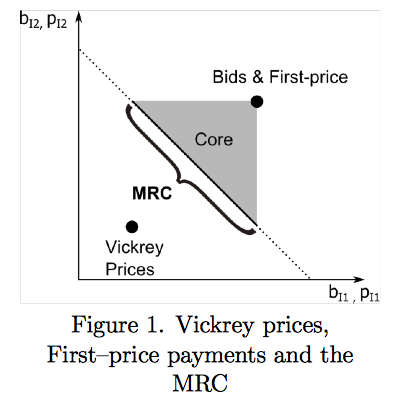
\includegraphics[width=50mm]{core1.png}
\label{fig:core2}
\end{figure}
\end{frame}


\begin{frame}
\frametitle{Coreに属するために}
\begin{itemize}\setlength{\parskip}{0.5em}
\item
じゃあ、コアに属するように真の評価額を引き出すためにはどうすれば良いのか?\pause
\begin{figure}
\centering
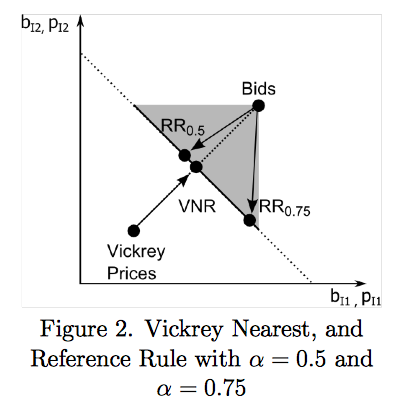
\includegraphics[width=40mm]{core2.png}
\label{fig:core}
\end{figure}
\item
The Vickrey Nearest Rule : VPをもとにコアを決定。
\item
The Reference Rule Auction : $b_{j}$をもとにコアを決定。
\end{itemize}
\end{frame}

\begin{frame}
\frametitle{The Vickrey Nearest Rule}
\begin{itemize}\setlength{\parskip}{0.5em}
\item
VPに最も近いMRC上の点を価格とする。
\item
数式で表すと以下の通り。
\begin{equation}
  P^{VNR}(b_{i1}, b_{i2}, b_{j}) = \begin{cases}
    (s_{i1}, s_{i2}, 0) & (b_{i1} + b_{i2} >= b_{j},and \\ & s_{i1},s_{i2} > 0) \\
    (b_{j}, 0, 0) & (b_{i1} <= b_{j} + b_{i2})\\
    (0, b_{j}, 0) & (b_{i2} <= b_{j} + b_{i1})\\
    (0, 0, b_{i1} + b_{i2}) & (b_{i1} + b_{i2} < b_{j})
  \end{cases}
\end{equation}
\begin{equation}
s_{i1} = (1/2)(b_{i1} + b_{j} - b_{i2})
\end{equation}
\begin{equation}
s_{i2} = (1/2)(b_{i2} + b_{j} - b_{i1})
\end{equation}

\end{itemize}
\end{frame}

\begin{frame}
\frametitle{The Reference Rule Auction}
\begin{itemize}\setlength{\parskip}{0.5em}
\item
パラメーター$\alpha$によってMRC上で価格を決める。
\item
数式で表すと以下の通り。
\begin{equation}
  P^{RR}(b_{i1}, b_{i2}, b_{j}) = \begin{cases}
    (r_{i1}, r_{i2}, 0) & (b_{i1} + b_{i2} >= b_{j},and \\ & r_{i1} < b_{i1},and ,r_{i2} < b_{i2}) \\
    (b_{j} - b_{i2}, b_{i2}, 0) & (b_{i1} + b_{i2} >= b_{j},and \\ & r_{i1} < b_{i1},and,  r_{i2} > b_{i2})\\
    (b_{i1}, b_{j} - b_{i1}, 0) & (b_{i1} + b_{i2} >= b_{j},and \\ & r_{i1} > b_{i1},and,  r_{i2} < b_{i2})\\
    (0, 0, b_{i1} + b_{i2}) & (b_{i1} + b_{i2} < b_{j})
  \end{cases}
\end{equation}
\begin{equation}
r_{i1} = \alpha  b_{j}
\end{equation}
\begin{equation}
r_{i2} = (1-\alpha)  b_{j}
\end{equation}
\end{itemize}
\end{frame}

\subsection{実験デザイン比較}
\begin{frame}
\frametitle{どれが1番良いのか?}
\begin{itemize}\setlength{\parskip}{0.5em}
\item
Revenue, Surplus, Efficiencyという3つの観点で比較する。\pause
\item
理論上、Ausubel and Baranov(2010)によって、revenue rankingは\\
\pause
1位VickreyAuction\\
2位FirstPrice\\
3位VNR, RR(0.50)\\
らしい。\pause
\item
さて本当なのかどうか。\pause
\item
先ほど行った実験のデータで調べてみる。
\end{itemize}
\end{frame}

\begin{frame}
\frametitle{論文でのデータ}
\begin{figure}
\centering
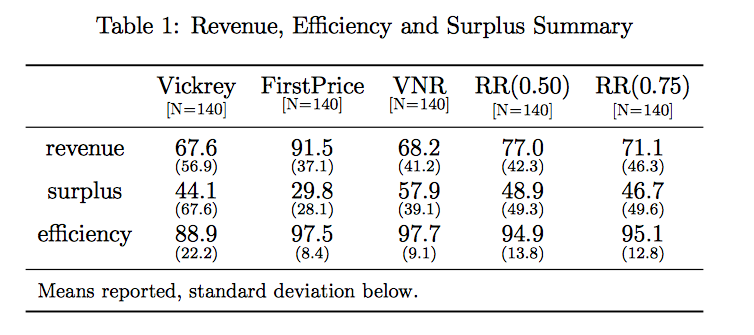
\includegraphics[width=120mm]{result.png}
\label{fig:result}
\end{figure}
\begin{itemize}\setlength{\parskip}{0.5em}
\pause
\item
FirstPriceが1番高い収入をもたらす!!
\end{itemize}
\end{frame}

\section{まとめ}
\subsection{結論}
\begin{frame}
\frametitle{結論}
\begin{itemize}\setlength{\parskip}{0.5em}
\item
世の中で広く扱われているFirstPriceAuction。\pause
\item
しかし、これは効率性を損なっているのではないかとの批判も多い制度でもある。\pause
\item
普通のオークションはこれでもいいけど、高い値段でのオークションは別の実験デザインに変更してちゃんと考えてみたほうが良いのでは?という意見も多々ある。\pause
\item
しかし、この論文において今まで理論上捉えられていたRevenue-rankingを覆し、FirstPriceAuctionは実はかなり優秀な制度であることを証明した!\pause
\item
みなさんもこのシンプルかつ優れているFirstPriceAuctionを使いましょう!
\end{itemize}
\end{frame}


\subsection{今後の課題}
\begin{frame}
\frametitle{今後の課題}
\begin{itemize}\setlength{\parskip}{0.5em}
\item
willowの使い方が一目で分かるような簡潔で美しいコードを書く。(公共財供給ゲーム)\pause
\item
Pandasを使ったデータ分析プログラムをセットで作っておく。\pause
\item
人が足りない時にコンピューターが相手をしてくれるようにコード内にエージェントを組み込む。
\end{itemize}
\end{frame}

\subsection{参考文献}
\begin{frame}
\frametitle{参考文献}
\begin{itemize}\setlength{\parskip}{0.5em}
\item
『Auction For Complements - An Experimental Analysis』(Daniel Marszalec,2014)\\
URL : http://www.cirje.e.u-tokyo.ac.jp/research/\\
workshops/micro/micropaper14/micro1021.pdf
\end{itemize}
\end{frame}


\end{document}